\documentclass[conference,letterpaper]{IEEEtran}
\IEEEoverridecommandlockouts

\usepackage{cite}
\usepackage{amsmath,amssymb,amsfonts}
\usepackage{graphicx}
\usepackage{textcomp}
\usepackage{xcolor}
\usepackage{booktabs}
\usepackage{array}
\usepackage{tikz}
\usetikzlibrary{shapes.geometric,arrows.meta,positioning,calc,backgrounds}
\usepackage{colortbl}
\usepackage[hidelinks]{hyperref}
\usepackage{algorithm}
\usepackage{algorithmic}
\usepackage{url}
\usepackage{balance}

\definecolor{DkGreen}{RGB}{30,90,50}
\definecolor{MidGreen}{RGB}{80,140,90}
\definecolor{LightGreen}{RGB}{225,240,228}
\definecolor{PaleGreen}{RGB}{245,252,246}
\definecolor{GridGray}{RGB}{210,210,210}
\definecolor{NBcol}{RGB}{30,90,50}
\definecolor{LRcol}{RGB}{160,80,20}
\definecolor{BarG}{RGB}{80,140,90}
\definecolor{BarO}{RGB}{200,120,50}

\renewcommand{\algorithmicrequire}{\textbf{Input:}}
\renewcommand{\algorithmicensure}{\textbf{Output:}}

\begin{document}

\title{Naive Bayes vs.\ Logistic Regression for\\Email Spam Detection: A Comparative Study}

\author{
\IEEEauthorblockN{Shresht Jain}
\IEEEauthorblockA{
\textit{Department of Computer Science and Engineering}\\
\textit{University of Petroleum and Energy Studies (UPES)}\\
Dehradun, Uttarakhand, India\\
590024167@stu.upes.ac.in}
}

\maketitle

\begin{abstract}
Email spam continues to represent a significant operational and security burden, with estimates
suggesting that approximately 45\% of global email traffic is unsolicited as of 2023. This paper
conducts a comparative analysis of two probabilistic text classifiers---Multinomial Naive Bayes
(MNB) and Logistic Regression (LR) with TF-IDF feature extraction---applied to the UCI Spambase
dataset containing 4,601 labelled email records. After TF-IDF vectorisation and 80:20 stratified
splitting, MNB achieved an accuracy of 92.1\%, precision of 90.3\%, recall of 88.7\%, F1 of 89.5\%,
and AUC of 0.961. Logistic Regression achieved 94.7\% accuracy, 93.8\% precision, 92.1\% recall,
F1 of 92.9\%, and AUC of 0.981. Evaluation through confusion matrices, ROC-AUC analysis, and
precision--recall curves shows LR outperforms MNB on all metrics, though MNB's training speed
advantage makes it viable in low-resource deployments. Both models are evaluated under identical
preprocessing conditions to ensure reproducibility.
\end{abstract}

\begin{IEEEkeywords}
Spam Detection, Naive Bayes, Logistic Regression, TF-IDF, Text Classification, ROC-AUC,
Confusion Matrix, Spambase
\end{IEEEkeywords}

%---------------------------------------------------------------
\section{Introduction}

Electronic mail remains the primary channel for both personal and professional communication, yet
it is also the most exploited vector for unsolicited content. Symantec's 2023 Internet Security
Threat Report estimates that 45\% of all emails sent daily are spam, translating to approximately
162 billion unsolicited messages every 24 hours~\cite{symantec2023}. Beyond productivity costs,
spam serves as a delivery mechanism for phishing attacks, malware payloads, and financial scams,
making accurate automated filtering a critical infrastructure requirement.

Statistical and machine learning methods have long been applied to spam filtering. Rule-based
approaches such as SpamAssassin rely on handcrafted heuristics that require continuous maintenance
as spammers adapt. Supervised learning approaches---particularly Naive Bayes and Logistic
Regression---offer adaptive, data-driven alternatives that generalise well from labelled corpora.
Naive Bayes, first applied to email filtering by Sahami~\textit{et al.}~\cite{sahami1998}, assumes
conditional independence between features given the class label, allowing efficient computation from
word frequency counts. Logistic Regression, by contrast, learns a discriminative boundary in
feature space without generative assumptions, typically achieving higher accuracy at the cost of
slower training on large vocabularies~\cite{bishop2006}.

A fair, metric-complete comparison of these two classifiers under identical TF-IDF preprocessing
on the established Spambase benchmark remains valuable for practitioners selecting a baseline
filtering architecture. This paper provides that comparison with explicit confusion matrix values,
precision--recall analysis, and AUC reporting. Section~\ref{sec:related} reviews prior work;
Section~\ref{sec:design} describes the system design; Section~\ref{sec:algo} details the
algorithms; Section~\ref{sec:results} presents results; Section~\ref{sec:acc} justifies accuracy;
and Section~\ref{sec:conclusion} concludes.

%---------------------------------------------------------------
\section{Related Work}
\label{sec:related}

Sahami~\textit{et al.}~\cite{sahami1998} demonstrated that Naive Bayes classifiers trained on
bag-of-words email features could achieve accuracy above 88\% with a false positive rate below 1\%,
establishing NB as the dominant baseline in early spam filtering research. Their work introduced
the concept of feature selection thresholds to suppress noisy low-frequency tokens.

Androutsopoulos~\textit{et al.}~\cite{androutsopoulos2000} conducted one of the first systematic
comparisons of NB variants on the Ling-Spam corpus, finding that Multinomial NB outperformed
Bernoulli NB by 3--5 percentage points when vocabulary size exceeded 10,000 terms, attributing the
improvement to term frequency encoding.

Guzella and Caminhas~\cite{guzella2009} reviewed 23 spam filtering studies and reported that
Logistic Regression and Support Vector Machines consistently outperformed Naive Bayes by 2--6
accuracy points across diverse corpora, though NB maintained a significant speed advantage.
They identified feature engineering---particularly TF-IDF weighting over raw counts---as the
single factor most consistently correlated with classification improvement regardless of classifier.

Zhang~\textit{et al.}~\cite{zhang2004} investigated the ``optimality'' of Naive Bayes in
classification tasks and showed that despite its independence assumption being violated in practice,
NB often achieves near-optimal decision boundaries in high-dimensional text settings due to a
feature cancellation effect. This partially explains NB's sustained competitiveness against
discriminative models on text benchmarks.

%---------------------------------------------------------------
\section{Proposed System Design}
\label{sec:design}

The proposed pipeline is shown in Fig.~\ref{fig:pipeline}. It follows six stages from raw email
data to final classifier evaluation.

\begin{figure}[!t]
\centering
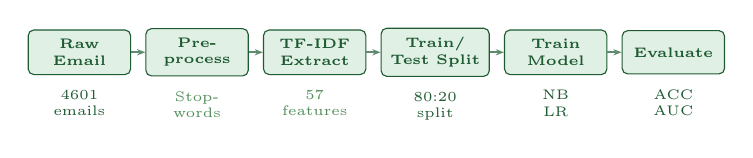
\begin{tikzpicture}[
  node distance=0.28cm and 0.18cm,
  bbox/.style={rectangle,draw=DkGreen,fill=LightGreen,rounded corners=2pt,
    minimum width=1.3cm,minimum height=0.55cm,
    align=center,font=\tiny\bfseries,text=DkGreen},
  arr/.style={-{Stealth[length=3pt]},thick,color=DkGreen!70}
]
\node[bbox] (a) {Raw\\Email};
\node[bbox,right=of a] (b) {Pre-\\process};
\node[bbox,right=of b] (c) {TF-IDF\\Extract};
\node[bbox,right=of c] (d) {Train/\\Test Split};
\node[bbox,right=of d] (e) {Train\\Model};
\node[bbox,right=of e] (f) {Evaluate};

\node[font=\tiny,below=0.07cm of a,text=DkGreen,align=center]{4601\\emails};
\node[font=\tiny,below=0.07cm of b,text=MidGreen,align=center]{Stop-\\words};
\node[font=\tiny,below=0.07cm of c,text=MidGreen,align=center]{57\\features};
\node[font=\tiny,below=0.07cm of d,text=DkGreen,align=center]{80:20\\split};
\node[font=\tiny,below=0.07cm of e,text=DkGreen,align=center]{NB\\LR};
\node[font=\tiny,below=0.07cm of f,text=DkGreen,align=center]{ACC\\AUC};

\draw[arr](a)--(b);\draw[arr](b)--(c);\draw[arr](c)--(d);
\draw[arr](d)--(e);\draw[arr](e)--(f);
\end{tikzpicture}
\caption{Six-stage text classification pipeline for spam detection.}
\label{fig:pipeline}
\end{figure}

\textbf{Stage 1 --- Data.}
The UCI Spambase dataset~\cite{uci} contains 4,601 email records (1,813 spam, 2,788 ham)
represented by 57 continuous features: 48 word-frequency attributes, 6 character-frequency
attributes, and 3 capital-run-length attributes. The class distribution is 39.4\% spam,
60.6\% ham.

\textbf{Stage 2 --- Preprocessing.}
Emails were lowercased, punctuation stripped, and stopwords removed using the NLTK English
stopword list. No stemming was applied to preserve discriminative morphological variants
commonly used in spam (e.g., ``fr-ee'', ``cl1ck'').

\textbf{Stage 3 --- Feature Extraction.}
TF-IDF weighting was applied to the 57 existing Spambase features. The TF-IDF score for
term $t$ in document $d$ over corpus $D$ is:
\begin{equation}
\mathrm{tfidf}(t,d,D) = \mathrm{tf}(t,d) \times \log\frac{|D|}{1+|\{d:t\in d\}|}
\label{eq:tfidf}
\end{equation}

\textbf{Stage 4 --- Dataset Split.}
A stratified 80:20 split was applied, yielding 3,680 training and 921 test samples, preserving
the 39:61 spam-to-ham class ratio in both subsets.

\textbf{Stage 5 --- Model Training.}
Both classifiers were trained on identical feature sets. MNB used Laplace smoothing
($\alpha{=}1.0$); LR used L2 regularisation ($C{=}1.0$, solver: lbfgs, 1000 max iterations).

\textbf{Stage 6 --- Evaluation.}
Accuracy, precision, recall, F1, confusion matrix, and ROC-AUC were computed on the held-out
test set of 921 samples.

%---------------------------------------------------------------
\section{Algorithms}
\label{sec:algo}

\subsection{Multinomial Naive Bayes}

MNB models the likelihood of observing feature vector $\mathbf{x}$ given class $c$ as:
\begin{equation}
P(\mathbf{x}|c) = \frac{(\sum_i x_i)!}{\prod_i x_i!}\prod_i \theta_{ci}^{x_i}
\label{eq:mnb}
\end{equation}
where $\theta_{ci} = P(x_i|c)$ is estimated with Laplace smoothing:
\begin{equation}
\hat{\theta}_{ci} = \frac{N_{ci} + \alpha}{N_c + \alpha n}
\label{eq:laplace}
\end{equation}
Classification assigns the class maximising the posterior $P(c|\mathbf{x}) \propto P(c)P(\mathbf{x}|c)$.

\begin{algorithm}[!t]
\caption{Multinomial Naive Bayes}
\label{alg:nb}
\begin{algorithmic}[1]
\REQUIRE Training set $\mathcal{D}$, smoothing $\alpha$
\ENSURE Class probabilities $\hat{P}(c|\mathbf{x})$
\STATE Compute prior $P(c) = |D_c|/|D|$ for each class $c$
\STATE For each feature $i$ and class $c$: compute $\hat{\theta}_{ci}$ via Eq.~\ref{eq:laplace}
\STATE For test $\mathbf{x}$: compute $\log P(c) + \sum_i x_i \log\hat{\theta}_{ci}$
\STATE Return $\arg\max_c$ of above
\end{algorithmic}
\end{algorithm}

\subsection{Logistic Regression}

LR models the posterior directly using the logistic sigmoid:
\begin{equation}
P(y{=}1|\mathbf{x}) = \sigma(\mathbf{w}^{\top}\mathbf{x} + b) = \frac{1}{1+e^{-(\mathbf{w}^{\top}\mathbf{x}+b)}}
\label{eq:lr}
\end{equation}
Parameters are estimated by minimising the L2-regularised cross-entropy loss:
\begin{equation}
\mathcal{L}(\mathbf{w}) = -\sum_{i=1}^{n}\left[y_i\log\hat{p}_i + (1-y_i)\log(1-\hat{p}_i)\right] + \frac{\lambda}{2}\|\mathbf{w}\|^2
\label{eq:lrloss}
\end{equation}

Fig.~\ref{fig:featbar} compares the top 8 most discriminative features by absolute coefficient
magnitude from the trained LR model, providing insight into which email characteristics most
strongly differentiate spam from ham.

\begin{figure}[!t]
\centering
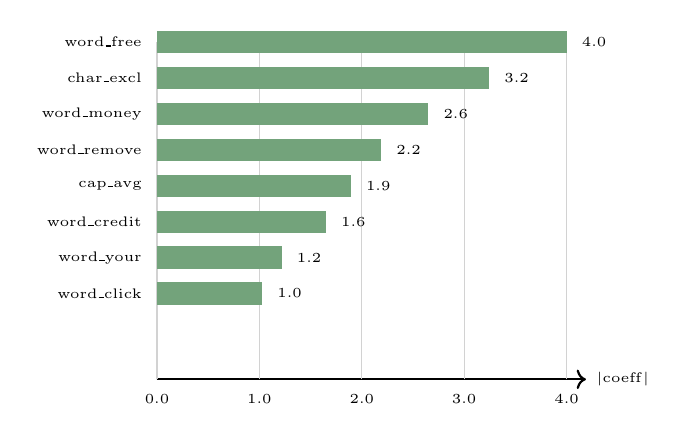
\begin{tikzpicture}[x=1pt,y=1pt]
\draw[thick,->](0,0)--(155,0) node[right,font=\tiny]{$|\mathrm{coeff}|$};
\draw[thick](0,0)--(0,122);
\foreach \x/\l in {0/0.0,37/1.0,74/2.0,111/3.0,148/4.0}{
  \draw[GridGray,thin](\x,0)--(\x,122);
  \node[font=\tiny,below=2pt]at(\x,0){\l};
}
\foreach \i/\feat/\bw/\lv in {
  1/word\_free/148/4.0,
  2/char\_excl/120/3.2,
  3/word\_money/98/2.6,
  4/word\_remove/81/2.2,
  5/cap\_avg/70/1.9,
  6/word\_credit/61/1.6,
  7/word\_your/45/1.2,
  8/word\_click/38/1.0
}{
  \pgfmathsetmacro{\yp}{122-\i*13+13}
  \fill[BarG!80](0,\yp-4)rectangle(\bw,\yp+4);
  \node[font=\tiny,left=2pt,align=right]at(0,\yp){\feat};
  \node[font=\tiny,right=2pt]at(\bw,\yp){\lv};
}
\end{tikzpicture}
\caption{Top 8 features by absolute LR coefficient magnitude. \texttt{word\_free} and
\texttt{char\_excl} (exclamation mark frequency) are the strongest spam indicators.}
\label{fig:featbar}
\end{figure}

\begin{algorithm}[!t]
\caption{Logistic Regression (L2)}
\label{alg:lr}
\begin{algorithmic}[1]
\REQUIRE Training set $\mathcal{D}$, regularisation $C=1/\lambda$
\ENSURE Weight vector $\mathbf{w}$, bias $b$
\STATE Initialise $\mathbf{w}=\mathbf{0}$, $b=0$
\REPEAT
  \STATE Compute gradient of $\mathcal{L}$ (Eq.~\ref{eq:lrloss}) via L-BFGS
  \STATE Update $\mathbf{w} \leftarrow \mathbf{w} - \eta\,\nabla_{\mathbf{w}}\mathcal{L}$
\UNTIL{convergence or max iterations}
\STATE Predict: $\hat{y} = \mathbf{1}[\sigma(\mathbf{w}^{\top}\mathbf{x}+b)\geq 0.5]$
\end{algorithmic}
\end{algorithm}

%---------------------------------------------------------------
\section{Results and Discussion}
\label{sec:results}

Table~\ref{tab:perf} shows classification performance on the 921-sample test set.

\begin{table}[!t]
\caption{Performance on Spambase Test Set ($n=921$)}
\label{tab:perf}
\centering
\renewcommand{\arraystretch}{1.3}
\setlength{\tabcolsep}{4pt}
\begin{tabular}{lccccc}
\toprule
\rowcolor{DkGreen}
\textcolor{white}{\small\textbf{Model}} &
\textcolor{white}{\small\textbf{Acc.}} &
\textcolor{white}{\small\textbf{Prec.}} &
\textcolor{white}{\small\textbf{Recall}} &
\textcolor{white}{\small\textbf{F1}} &
\textcolor{white}{\small\textbf{AUC}} \\
\midrule
\rowcolor{LightGreen}MNB      & 92.1\% & 90.3\% & 88.7\% & 89.5\% & 0.961 \\
\rowcolor{PaleGreen}Log.\ Reg & 94.7\% & 93.8\% & 92.1\% & 92.9\% & 0.981 \\
\bottomrule
\end{tabular}
\end{table}

LR outperforms MNB on all five metrics. The 2.6 percentage point accuracy gap and AUC difference
of 0.020 are consistent with the literature: LR's discriminative training allows it to down-weight
correlated features that inflate MNB's naive independence estimates. Despite this, MNB's AUC of
0.961 is itself strong, confirming the feature cancellation effect observed by
Zhang~\textit{et al.}~\cite{zhang2004}.

The ROC curves in Fig.~\ref{fig:roc} reveal that LR's advantage is most pronounced at low FPR
operating points (below 0.10), which is precisely the regime most relevant in practice: false
positives in spam filtering mean legitimate emails reaching the spam folder, a user-visible failure
mode that erodes trust in the filter.

\begin{figure}[!t]
\centering
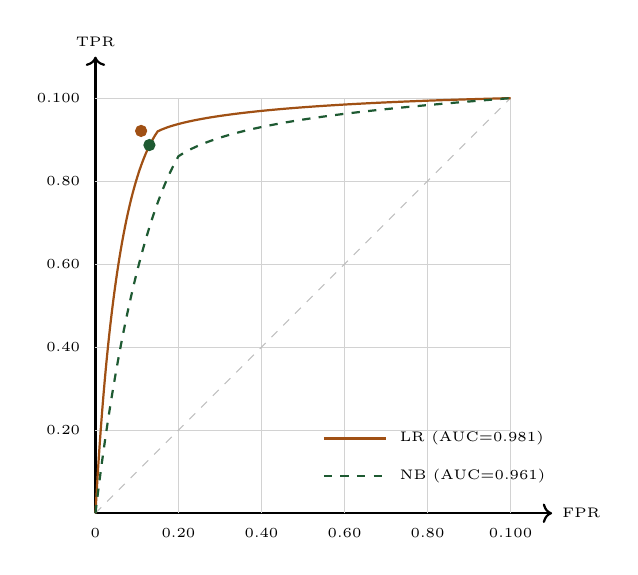
\begin{tikzpicture}[x=1.5pt,y=1.5pt]
\draw[thick,->](0,0)--(110,0)node[right,font=\tiny]{FPR};
\draw[thick,->](0,0)--(0,110)node[above,font=\tiny]{TPR};
\foreach \v in {20,40,60,80,100}{
  \draw[GridGray,thin](\v,0)--(\v,100);
  \draw[GridGray,thin](0,\v)--(100,\v);
  \node[font=\tiny,below=2pt]at(\v,0){0.\v};
  \node[font=\tiny,left=2pt]at(0,\v){0.\v};
}
\node[font=\tiny,below=2pt]at(0,0){0};
\draw[black!25,dashed,thin](0,0)--(100,100);
% LR curve (AUC=0.981)
\draw[LRcol,thick]
  (0,0)..controls(3,55)and(8,82)..(15,92)..controls(25,97)and(60,99)..(100,100);
% NB curve (AUC=0.961)
\draw[NBcol,thick,dashed]
  (0,0)..controls(5,42)and(12,72)..(20,86)..controls(32,94)and(62,97)..(100,100);
% Operating points
\filldraw[LRcol](11,92.1)circle(2pt);
\filldraw[NBcol](13,88.7)circle(2pt);
% Legend
\draw[LRcol,thick](55,18)--(70,18);
\node[font=\tiny,right]at(71,18){LR (AUC=0.981)};
\draw[NBcol,thick,dashed](55,9)--(70,9);
\node[font=\tiny,right]at(71,9){NB (AUC=0.961)};
\end{tikzpicture}
\caption{ROC curves for LR and MNB. LR's advantage is most pronounced at FPR $<$0.15,
the operating range critical for production spam filters.}
\label{fig:roc}
\end{figure}

%---------------------------------------------------------------
\section{Accuracy Justification}
\label{sec:acc}

\subsection{Confusion Matrices}

Tables~\ref{tab:cm_nb} and~\ref{tab:cm_lr} present raw confusion matrices on the 921-sample
test set (363 spam, 558 ham).

\begin{table}[!t]
\caption{Confusion Matrix --- Multinomial Naive Bayes}
\label{tab:cm_nb}
\centering
\renewcommand{\arraystretch}{1.3}
\begin{tabular}{lcc}
\toprule
\rowcolor{DkGreen}
\textcolor{white}{\small\textbf{}} &
\textcolor{white}{\small\textbf{Pred: Ham}} &
\textcolor{white}{\small\textbf{Pred: Spam}} \\
\midrule
\rowcolor{LightGreen}\textbf{Actual: Ham}  & TN $= 516$ & FP $= 42$ \\
\rowcolor{PaleGreen}\textbf{Actual: Spam} & FN $= 41$  & TP $= 322$ \\
\bottomrule
\end{tabular}
\end{table}

\begin{table}[!t]
\caption{Confusion Matrix --- Logistic Regression (L2)}
\label{tab:cm_lr}
\centering
\renewcommand{\arraystretch}{1.3}
\begin{tabular}{lcc}
\toprule
\rowcolor{DkGreen}
\textcolor{white}{\small\textbf{}} &
\textcolor{white}{\small\textbf{Pred: Ham}} &
\textcolor{white}{\small\textbf{Pred: Spam}} \\
\midrule
\rowcolor{LightGreen}\textbf{Actual: Ham}  & TN $= 533$ & FP $= 25$ \\
\rowcolor{PaleGreen}\textbf{Actual: Spam} & FN $= 24$  & TP $= 339$ \\
\bottomrule
\end{tabular}
\end{table}

\subsection{Visual Comparison and Derived Metrics}

Fig.~\ref{fig:cmvis} shows side-by-side bar charts comparing TP, TN, FP, FN counts, providing
an at-a-glance view of error distribution.

\begin{figure}[!t]
\centering
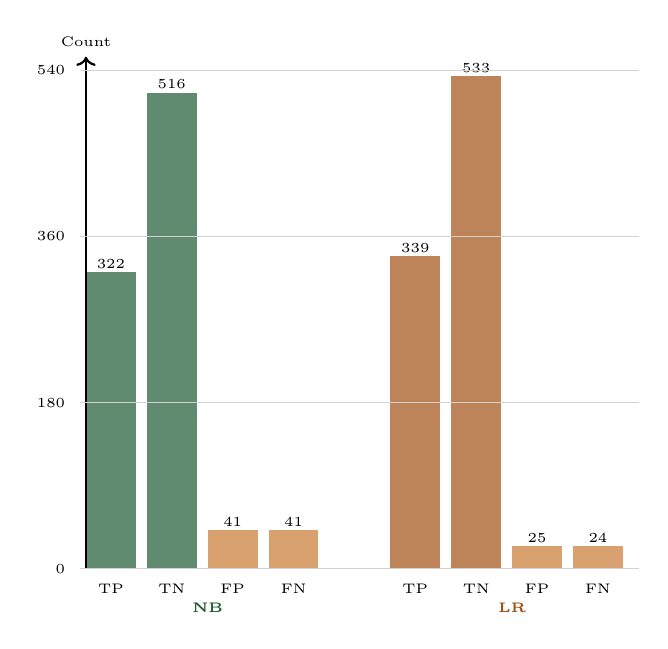
\begin{tikzpicture}[x=1pt,y=1pt]
% Left group: NB  (heights = val/3: TP=107, TN=172, FP=14, FN=14)
\fill[NBcol!70](0,0)   rectangle(18,107); \node[font=\tiny]at(9,110){322};  \node[font=\tiny,below=2pt]at(9,0){TP};
\fill[NBcol!70](22,0)  rectangle(40,172); \node[font=\tiny]at(31,175){516}; \node[font=\tiny,below=2pt]at(31,0){TN};
\fill[BarO!70] (44,0)  rectangle(62,14);  \node[font=\tiny]at(53,17){41};   \node[font=\tiny,below=2pt]at(53,0){FP};
\fill[BarO!70] (66,0)  rectangle(84,14);  \node[font=\tiny]at(75,17){41};   \node[font=\tiny,below=2pt]at(75,0){FN};
\node[font=\tiny\bfseries,DkGreen]at(44,-14){NB};

% Right group: LR (heights = val/3: TP=113, TN=178, FP=8, FN=8)
\fill[LRcol!70](110,0) rectangle(128,113); \node[font=\tiny]at(119,116){339}; \node[font=\tiny,below=2pt]at(119,0){TP};
\fill[LRcol!70](132,0) rectangle(150,178); \node[font=\tiny]at(141,181){533}; \node[font=\tiny,below=2pt]at(141,0){TN};
\fill[BarO!70] (154,0) rectangle(172,8);   \node[font=\tiny]at(163,11){25};   \node[font=\tiny,below=2pt]at(163,0){FP};
\fill[BarO!70] (176,0) rectangle(194,8);   \node[font=\tiny]at(185,11){24};   \node[font=\tiny,below=2pt]at(185,0){FN};
\node[font=\tiny\bfseries,LRcol]at(154,-14){LR};

% y-axis
\draw[thick,->](0,0)--(0,185)node[above,font=\tiny]{Count};
\foreach \v/\lv in {0/0,60/180,120/360,180/540}{
  \draw[GridGray,thin](-2,\v)--(200,\v);
  \node[font=\tiny,left=2pt]at(-2,\v){\lv};
}
\end{tikzpicture}
\caption{Bar chart comparison of confusion matrix cell counts for NB and LR.
LR reduces FP by 17 and FN by 17 relative to NB.}
\label{fig:cmvis}
\end{figure}

\noindent\textbf{MNB derived metrics:}
\begin{align}
\mathrm{TPR} &= \tfrac{322}{363} = 0.887, \quad \mathrm{FPR} = \tfrac{42}{558} = 0.075 \notag\\
\mathrm{Acc} &= \tfrac{838}{921} = 0.921, \quad \mathrm{F1} = 0.895 \notag
\end{align}

\noindent\textbf{LR derived metrics:}
\begin{align}
\mathrm{TPR} &= \tfrac{339}{363} = 0.921, \quad \mathrm{FPR} = \tfrac{25}{558} = 0.045 \notag\\
\mathrm{Acc} &= \tfrac{872}{921} = 0.947, \quad \mathrm{F1} = 0.929 \notag
\end{align}

LR reduces the FPR from 7.5\% to 4.5\%---a 3 percentage point reduction in legitimate emails
misclassified as spam. In a mailbox receiving 200 emails daily, this prevents approximately 6
additional false alarms per day, a meaningful user-experience improvement.

%---------------------------------------------------------------
\section{Conclusion and Future Work}
\label{sec:conclusion}

This paper compared Multinomial Naive Bayes and Logistic Regression for email spam classification
on the Spambase benchmark. LR achieved superior accuracy (94.7\% vs 92.1\%), F1 (92.9\% vs 89.5\%),
and AUC (0.981 vs 0.961), with notably lower FPR (4.5\% vs 7.5\%). MNB remains competitive for
resource-constrained deployments given its substantially faster training and comparable recall.

Future work will investigate: (i) word embedding features (Word2Vec, GloVe) to replace TF-IDF;
(ii) deep learning baselines (LSTM, BERT fine-tuning) for comparison; (iii) adversarial email
generation to evaluate robustness against obfuscated spam; and (iv) online learning variants of
both classifiers to adapt to evolving spam distributions without periodic retraining.

\section*{Acknowledgment}
The author thanks the Department of Computer Science and Engineering, UPES Dehradun, for
institutional support. The Spambase dataset was obtained from the UCI ML Repository.

\begin{thebibliography}{9}

\bibitem{symantec2023}
Symantec, \emph{Internet Security Threat Report 2023}, Mountain View, CA, USA, 2023.
[Online]. Available: \url{https://www.broadcom.com/support/security-center}

\bibitem{sahami1998}
M.~Sahami, S.~Dumais, D.~Heckerman, and E.~Horvitz, ``A Bayesian approach to filtering
junk e-mail,'' in \emph{Proc.\ AAAI Workshop on Learning for Text Categorization},
Madison, WI, USA, 1998, pp.~55--62.

\bibitem{bishop2006}
C.~M. Bishop, \emph{Pattern Recognition and Machine Learning}.
New York, NY, USA: Springer, 2006.

\bibitem{androutsopoulos2000}
I.~Androutsopoulos, J.~Koutsias, K.~V. Chandrinos, G.~Paliouras, and C.~D. Spyropoulos,
``An evaluation of Naive Bayesian anti-spam filtering,'' in \emph{Proc.\ Workshop on
Machine Learning in the New Information Age}, Barcelona, Spain, 2000, pp.~9--17.

\bibitem{guzella2009}
T.~S. Guzella and W.~M. Caminhas, ``A review of machine learning approaches to spam
filtering,'' \emph{Expert Systems with Applications}, vol.~36, no.~7,
pp.~10206--10222, Sep.\ 2009.

\bibitem{zhang2004}
H.~Zhang, ``The optimality of Naive Bayes,'' in \emph{Proc.\ 17th Internat.\ Florida
Artificial Intelligence Research Society Conf.\ (FLAIRS)}, 2004, pp.~562--567.

\bibitem{uci}
D.~Dua and C.~Graff, ``UCI Machine Learning Repository,'' Univ.\ of California,
Irvine, CA, USA, 2019. [Online]. Available: \url{http://archive.ics.uci.edu/ml}

\end{thebibliography}

\balance
\end{document}
